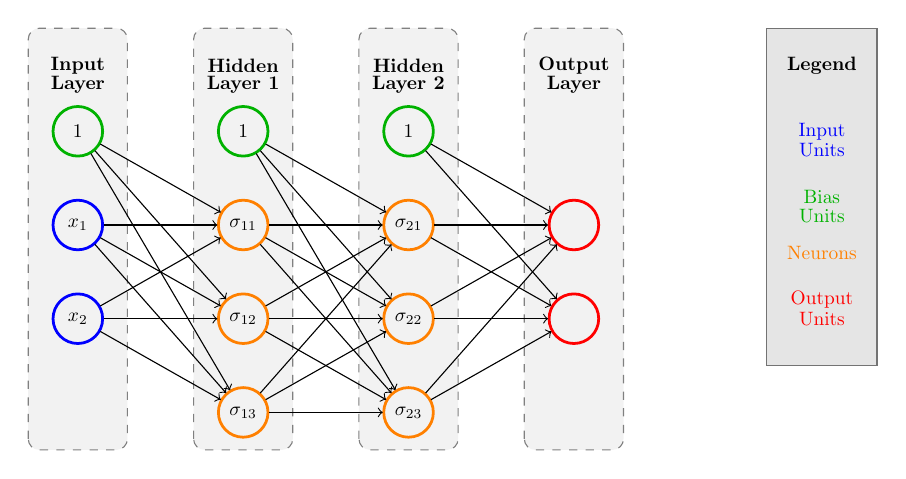
\begin{tikzpicture}[scale=0.7, every node/.style={scale=0.7}]
    %--------------------%
    % Parameters
    %--------------------%
    \def\layersep{3}
    \def\ysep{1.7}
    \def\circlesize{0.9cm}
    \def\labelshift{0.75}
    \def\woffset{5}
    \def\linethic{1.0pt}

    %--------------------%
    % Layer Rectangles
    %--------------------%
    % Input Layer Rectangle
    \draw[fill=gray!10, draw=gray, dashed, rounded corners] 
        (-0.9, -1.4*\ysep) rectangle (0.9, 3.1*\ysep);
    % Hidden 1 Rectangle
    \draw[fill=gray!10, draw=gray, dashed, rounded corners] 
        (\layersep-0.9, -1.4*\ysep) rectangle (\layersep+0.9, 3.1*\ysep);
    % Hidden 2 Rectangle
    \draw[fill=gray!10, draw=gray, dashed, rounded corners] 
        (2*\layersep-0.9, -1.4*\ysep) rectangle (2*\layersep+0.9, 3.1*\ysep);
    % Output Layer Rectangle
    \draw[fill=gray!10, draw=gray, dashed, rounded corners] 
        (3*\layersep-0.9, -1.4*\ysep) rectangle (3*\layersep+0.9, 3.1*\ysep);

    %--------------------%
    % Input Layer
    %--------------------%
    \node[draw=green!70!black, circle, minimum size=\circlesize, line width=\linethic] (theta0) at (0,2*\ysep) {1};
    \node[draw=blue ,circle, minimum size=\circlesize, line width=\linethic] (x1) at (0,1*\ysep) {$x_1$};
    \node[draw=blue ,circle, minimum size=\circlesize, line width=\linethic] (x2) at (0,0*\ysep) {$x_2$};

    %--------------------%
    % Layer 1
    %--------------------%
    \node[draw=green!70!black, circle, minimum size=\circlesize, line width=\linethic] (theta1) at (\layersep,2*\ysep) {1};
    \node[draw=orange ,circle, minimum size=\circlesize, line width=\linethic] (sigma11) at (\layersep,1*\ysep) {$\sigma_{11}$};
    \node[draw=orange ,circle, minimum size=\circlesize, line width=\linethic] (sigma12) at (\layersep,0*\ysep) {$\sigma_{12}$};
    \node[draw=orange ,circle, minimum size=\circlesize, line width=\linethic] (sigma13) at (\layersep,-1*\ysep) {$\sigma_{13}$};

    %--------------------%
    % Layer 2
    %--------------------%
    \node[draw=green!70!black ,circle, minimum size=\circlesize, line width=\linethic] (theta2) at (2*\layersep,2*\ysep) {1};
    \node[draw=orange ,circle, minimum size=\circlesize, line width=\linethic] (sigma21) at (2*\layersep,1*\ysep) {$\sigma_{21}$};
    \node[draw=orange ,circle, minimum size=\circlesize, line width=\linethic] (sigma22) at (2*\layersep,0) {$\sigma_{22}$};
    \node[draw=orange ,circle, minimum size=\circlesize, line width=\linethic] (sigma23) at (2*\layersep,-1*\ysep) {$\sigma_{23}$};

    %--------------------%
    % Output Layer
    %--------------------%
    \node[draw=red ,circle, minimum size=\circlesize, line width=\linethic] (out1) at (3*\layersep,1*\ysep) {};
    \node[draw=red ,circle, minimum size=\circlesize, line width=\linethic] (out2) at (3*\layersep,0*\ysep) {};

    %--------------------%
    % Connections
    %--------------------%
    % Input to Layer 1
    \draw[->] (theta0) -- node[above,midway]{} (sigma11);
    \draw[->] (theta0) -- node[above,midway]{} (sigma12);
    \draw[->] (theta0) -- node[above,midway]{} (sigma13);
    \draw[->] (x1) -- node[above,midway]{} (sigma11);
    \draw[->] (x1) -- node[above,midway]{} (sigma12);
    \draw[->] (x1) -- node[above,midway]{} (sigma13);
    \draw[->] (x2) -- node[above,midway]{} (sigma11);
    \draw[->] (x2) -- node[above,midway]{} (sigma12);
    \draw[->] (x2) -- node[above,midway]{} (sigma13);

    % Layer 1 to Layer 2
    \draw[->] (theta1) -- node[above,midway]{} (sigma21);
    \draw[->] (theta1) -- node[above,midway]{} (sigma22);
    \draw[->] (theta1) -- node[above,midway]{} (sigma23);
    \draw[->] (sigma11) -- node[above,midway]{} (sigma21);
    \draw[->] (sigma11) -- node[above,midway]{} (sigma22);
    \draw[->] (sigma11) -- node[above,midway]{} (sigma23);
    \draw[->] (sigma12) -- node[above,midway]{} (sigma21);
    \draw[->] (sigma12) -- node[above,midway]{} (sigma22);
    \draw[->] (sigma12) -- node[above,midway]{} (sigma23);
    \draw[->] (sigma13) -- node[above,midway]{} (sigma21);
    \draw[->] (sigma13) -- node[above,midway]{} (sigma22);
    \draw[->] (sigma13) -- node[above,midway]{} (sigma23);

   % Layer 2 to Output Layer
    \draw[->] (theta2) -- node[above,midway]{} (out1);
    \draw[->] (theta2) -- node[above,midway]{} (out2);
    \draw[->] (sigma21) -- node[above,midway]{} (out1);
    \draw[->] (sigma21) -- node[above,midway]{} (out2);
    \draw[->] (sigma22) -- node[above,midway]{} (out1);
    \draw[->] (sigma22) -- node[above,midway]{} (out2);
    \draw[->] (sigma23) -- node[above,midway]{} (out1);
    \draw[->] (sigma23) -- node[above,midway]{} (out2);

    %--------------------%
    % Layer Labels
    %--------------------%
    \node at (0*\layersep, 2.7*\ysep) {\textbf{Input}};
    \node at (0*\layersep, 2.5*\ysep) {\textbf{Layer}};
    \node at (1*\layersep, 2.7*\ysep) {\textbf{Hidden}};
    \node at (1*\layersep, 2.5*\ysep) {\textbf{Layer 1}};
    \node at (2*\layersep, 2.7*\ysep) {\textbf{Hidden}};
    \node at (2*\layersep, 2.5*\ysep) {\textbf{Layer 2}};
    \node at (3*\layersep, 2.7*\ysep) {\textbf{Output}};
    \node at (3*\layersep, 2.5*\ysep) {\textbf{Layer}};

    %--------------------%
    % Legend
    %--------------------%
    \draw[fill=gray!20, draw=gray!90!black] 
        (4.5*\layersep-1, -0.5*\ysep) rectangle (4.5*\layersep+1, 3.1*\ysep);
    \node at (4.5*\layersep, 2.7*\ysep) {\textbf{Legend}};

    \node[text=blue] at (4.5*\layersep, 2.0*\ysep) {Input};
    \node[text=blue] at (4.5*\layersep, 1.8*\ysep) {Units};

    \node[text=green!70!black] at (4.5*\layersep, 1.3*\ysep) {Bias};
    \node[text=green!70!black] at (4.5*\layersep, 1.1*\ysep) {Units};

    \node[text=orange] at (4.5*\layersep, 0.7*\ysep) {Neurons};

    \node[text=red] at (4.5*\layersep, 0.2*\ysep) {Output};
    \node[text=red] at (4.5*\layersep, 0.0*\ysep) {Units};
\end{tikzpicture}
